\chapter{MULTI-OBSERVATORY SPECTRAL ANALYSIS OF SUPERSOFT X-RAY SOURCES} \label{chap:multi-obs}
    %\doublespacing
    \minitoc
    \emph{Abstract of chapter \ref{chap:multi-obs}}
    
    \section{Literature Review} \label{multi-obs:lit-rev}
    	Supersoft X-ray sources (SSS) represent an important class of celestial objects. They were initially recognized as a distinct class of intrinsically luminous X-ray sources by Trümper \textit{et al.} \cite{trumper1991x}, Greiner \textit{et al.} \cite{greiner1991rosat}, and Kahabka \textit{et al.} \cite{kahabka97}. These sources are classified based on their X-ray luminosities, which are typically around the Eddington limit ($\sim 10^{38}$ erg s$^{-1}$), indicating their exceptionally high brightness. However, their defining feature is their extremely soft X-ray spectra, with weak or negligible emission beyond $\sim 1$ keV and effective blackbody temperature no more than $\sim 100$ eV (or $\lesssim 1200$ kK) \cite{kahabka06}. The understanding of the spectral characteristics of SSS promises to pave the way for a deeper exploration of their role in the broader astrophysical landscape.
    	
    	SSS were initially observed by the Einstein Observatory during a soft X-ray survey of the Large Magellanic Cloud (LMC) by Long et al. in 1981 \cite{long81}. Over time, hundreds of objects exhibiting similar characteristics have been documented, many of which are considered candidates or confirmed members of this class. The catalog of SSS has expanded significantly, now encompassing sources not only within the LMC but also various other celestial bodies, including the Milky Way (MW), Small Magellanic Cloud (SMC), and Andromeda (M31) and numerous other galaxies \cite{kahabkatrumper1996,steinerdiaz1998,greiner2000,pietsch2003deep,di2003luminous,orio2010census,henze2010recent,sturm2012new,galiullin2021populations}.
    	
    	The relatively fewer detections of SSS within our galaxy, compared to other galaxies, may be attributed to significant interstellar extinction of soft X-rays. Situated at the edge of the MW and along its galactic plane, soft X-rays emitted by galactic SSS face considerable interstellar absorption. Suggestions have been made that SSS within the galactic plane must be within a distance of approximately 1 kpc to remain observable. Beyond this distance, interstellar absorption becomes sufficiently pronounced to render them undetectable \cite{van1992accreting}.
    	
    	The optical spectra of the SSS in the Magellanic Cloud galaxies exhibit similarities with those of low-mass X-ray binaries -- characterized by strong emission lines such as He II at 4686 \AA\ and hydrogen Balmer lines. Subsequent numerical calculations suggested that SSS could result from near-Eddington accretion onto neutron stars \cite{kylafis93}, although subsequent analyses favoured white dwarfs as the emitting objects for supersoft X-rays \cite{vandenHeuvel92}.
    	
    	Employing Stefan-Boltzmann's law with typical luminosity and effective temperature values for SSS, the estimated radius of the emitting object aligns with that of a white dwarf, supporting the hypothesis of accretion onto white dwarfs as the source of supersoft X-rays, akin to accreting neutron stars and black holes in classical X-ray binaries. Van den Heuvel proposed that white dwarfs with masses in the range $0.7–1.4\,M_\odot$ and mass accretion rates $\sim 1-5\times 10^{-7}\,M_\odot\text{ yr}^{-1}$ produce supersoft X-rays, assuming the mass-accretor as the white dwarf and the companion as a main-sequence or post-main-sequence star within specific mass ranges \cite{van1992accreting}. Studies by various groups have explored different types of nuclear burning due to mass accretion on white dwarfs, depending on the thermal history of the white dwarf and conditions required for nuclear ignition, typically involving critical envelope masses %$\Delta M_\text{crit}$
    sustaining high temperatures ($\sim 10^8$ K) and pressures ($\gtrsim 10^{18}-10^{20}$ g cm$^{-1}$ s$^{-2}$) for nuclear burning via the CNO cycle \cite{paczynski78,prialnik78,sion79,sienkiewicz80,nomoto82,fujimoto82a,fujimoto82b,iben82,prialnik95,macdonald83}. The steady state accretion rate, crucial for understanding the relationship between accretion and nuclear burning, has been investigated in early calculations \cite{paczynski80,iben82}, providing insights into the dynamics of hydrogen-rich matter accretion on white dwarfs. For a hydrogen-rich system, the steady state accretion rate was given to be \cite{hachisu2001}
		\begin{align}
			\dot{M}_\text{steady}\sim 3.7\times 10^{-7}\left( \dfrac{M_\text{WD}}{M_\odot}-0.4 \right)\,M_\odot\,\text{yr}^{-1} \label{eqn:steady-mass-accr}
		\end{align}
	
		The particular luminous galactic SSS known as MR Vel, and referred to as \source, was discovered by Motch \textit{et al.} \cite{motch1994} in the ROSAT Galactic Plane Survey (RGPS), which  is defined as the $|b|\leqslant 20\degree$ region of the ROSAT All Sky Survey. In the J2000 frame, the right ascension and declination of \source\ is 141.44042 and -47.96972 ($\alpha$=09 25 46.00, $\delta$=-47 58 17.4: as resolved by Simbad\footnote{\url{http://simbad.u-strasbg.fr/simbad/}}).
		
		\source\ was the brightest SSS candidate source in RGPS, with ROSAT PSPC hardness ratios of $HR1=0.96\pm 0.03$ and $HR2=-0.69\pm 0.03$. Fitting a blackbody to the ROSAT observations, a hydrogen column density in the range $n_H=(1.4-3.7)\times 10^{22}$ cm$^{-2}$ can be obtained. There is a considerable amount of uncertainty in current literature about its distance, with estimates ranging from 1 kpc to 10 kpc. Consulting Gaia Data Release 3\footnote{\url{https://www.cosmos.esa.int/web/gaia/data-release-3}}, one can find negligible parallax. This fact along with its high luminosity suggests that its distance is likely to be $>5$ kpc.
		
		Hartmann \textit{et al.} applied non-local thermodynamic equilibrium (NLTE) models, which included metal line opacities, to the spectrum extracted from the observations by BeppoSAX LECS of RX J0925 on January 25-26 1997 \cite{hartmann1999constraining}. They found that if a single model component is assumed for \source, a large discrepancy is observed between the model and data above 1.19 keV. The emission above $\sim 1.2$ kev (i.e. Ne IX edge) can be accounted for by adding another spectral model component, namely collisional ionization equilibrium.
		
		Higher resolution data obtained using the grating instruments on-board the Chandra and XMM-Newton observatories revealed complex structures in the spectra of \source. Such spectra show the presence of P Cygni profiles of Fe XVII and O VIII, which typically arise in a wind. Earlier, Bearda et al. (2002) and Motch et al. (2002) had come to the conclusion that the \source\ spectra, as observed by the Chandra HETGS and the XMM-Newton RGS, cannot be reproduced by LTE or NLTE model atmospheres \cite{beardaChandra2002AA,motchXmmNewton2002AA}, even though there is little clarity on the reason for this. Obtaining an acceptable fit for \source\ spectrum assumes crucial importance at this juncture. In the absence of a proper model describing the emission spectrum, it becomes impossible to calculate its parameters such as effective temperature and luminosity.
		
		In the present work, our primary objective was to identify a robust spectral model capable of providing an acceptable fit to the continuum spectrum of \source. To this end, we devised an approach wherein we analyse spectral data for \source\ obtained using multiple observatories. A motivation for harnessing such multi-observatory science data over an extended period was to mitigate potential biases associated with individual instruments and temporal variations in observational conditions, thereby enabling a systematic examination of the source's spectral characteristics, in an attempt to constrain the underlying physical processes driving the observed supersoft X-ray emission.
		
		The amalgamation of observations from diverse space observatories offered unique insights into the spectral evolution of the supersoft X-ray source over time, shedding light on its dynamic behavior and emission properties. Through rigorous spectral modeling and comparative analysis, we made an attempt to establish a robust framework for characterizing the continuum spectrum of the supersoft source, thereby enhancing our understanding of its astrophysical nature and evolutionary trends. A comprehensive investigation into recurrent SSS like \source\ is paramount due to the emerging recognition of SSS as progenitors of type Ia supernovae, which serve as crucial standard candles in cosmology. By delving deeper into the astrophysical mechanisms governing SSS, we can potentially enhance our ability to make precise predictions regarding the occurrence of type Ia supernovae and subsequently refine cosmological distance measurements.
    
    \section{Journal of Observations} \label{multi-obs:journal}
    	During the course of our investigation of the continuum spectrum of \source, we leveraged a comprehensive dataset comprising six observations conducted by four distinct space observatories spanning the years 1994 to 2019. We extracted spectral data within the range 0.2 -- 1.0 keV from each observation in this dataset. This afforded us the opportunity to apply a consistent spectral analysis approach across a broad temporal range and disparate instrumentation platforms.
    	
    	A summary of the observations used in this study, which included science data from Japan's ASCA \cite{ebisawaAsca2001ApJ}, NASA's Chandra \cite{beardaChandra2002AA}, ESA's XMM-Newton \cite{motchXmmNewton2002AA} and ISS' NICER \cite{orioNicer2022ApJ} observatories, is presented in table \ref{tab:obs-journal}.
    	
    	\begin{landscape}    	
    	\begin{table}[!htb]
	    	\centering
	    	\caption{Journal of observations}
	    	\label{tab:obs-journal}
			\begin{tabular}{ccccccc}
				\hline
				\textbf{\begin{tabular}[c]{@{}c@{}}Observation\\ (Obs. ID)\end{tabular}} & \textbf{\begin{tabular}[c]{@{}c@{}}Date\\ (yyyy-mm-dd)\end{tabular}} & \textbf{Observatory} & \textbf{Instrument} & \textbf{MJD}$^\dagger$ & \textbf{\begin{tabular}[c]{@{}c@{}}Exposure$^\ddagger$\\ (ks)\end{tabular}} & \textbf{Region (keV)} \\
				\hline
				{43036000}   & {1994-12-22} & {ASCA} & {SIS1}          & {49708.56} & {20.58} & {0.20--1.00} \\
				{644}        & {2000-11-14} & {Chandra} & {ACIS}       & {51862.92} & {57.40} & {0.40--1.00} \\
				{0111150101} & {2000-12-16} & {XMM-Newton} & {EPIC-pn} & {51894.46} & {61.10} & {0.30--1.00} \\
				{2611020101} & {2019-05-18} & {NICER} & {XTI}          & {58621.90} & {2.53} & {0.40--1.00}  \\
				{2611020102} & {2019-05-19} & {NICER} & {XTI}          & {58622.03} & {8.57} & {0.45--1.00}  \\
				{2611020103} & {2019-05-19} & {NICER} & {XTI}          & {58623.00} & {9.91} & {0.45--1.00}  \\
				\hline
			\end{tabular}
			
			\begin{minipage}{16cm}
				\vspace{0.1cm}
				\small $^\dagger$Modified Julian Date
				
				\small $^\ddagger$From HEASARC archival query results
			\end{minipage}
		\end{table}
		\end{landscape}
    
    \section{Data Reduction and Analysis} \label{multi-obs:red-analysis}
    	The raw data pertaining to all of the observations were downloaded using the online archival query interface at the \textit{High Energy Astrophysics Science Archive Research Center} (HEASARC)\footnote{\url{https://heasarc.gsfc.nasa.gov/db-perl/W3Browse/w3browse.pl}}. The data was reduced finally to \textit{Flexible Image Transport System} (FITS)\footnote{\url{https://fits.gsfc.nasa.gov/standard40/fits_standard40aa-le.pdf}} format using the software tools for the corresponding observatory with recommended settings in the relevant data analysis threads, wherever available. For the final analysis, a set of four files were generated for each of the observations. As a standard practice, these files were given the extensions as per a convention adopted by the authors as follows:
	    \begin{enumerate}
	    	\item Source spectrum, with file extension \texttt{.src}
	    	\item Background spectrum, with file extension \texttt{.bkg}
	    	\item Redistribution matrix file (RMF), with file extension \texttt{.rmf}
	    	\item Ancillary response file (ARF), with file extension \texttt{.arf}
	    \end{enumerate}
	    The above files were grouped using the FTOOLS task \texttt{grphha}\footnote{\url{https://heasarc.gsfc.nasa.gov/docs/heasarc/caldb/docs/memos/cal_sw_93_010/cal_sw_93_010.pdf}} to have an appropriate minimum number of counts per bin. The resulting spectrum sets were analysed using \textit{XSPEC} version 12.13.1.
    
    	\subsection{XMM-Newton EPIC-pn Data Reduction} \label{multi-obs:red-analysis:epic-pn}
    		The SSS \source\ was observed by all the instruments, viz. EPIC-MOS 1, EPIC-MOS 2, EPIC-pn and RGS, on-board ESA's XMM-Newton observatory for $\sim 52$ ks on 16 December 2000. Whereas, we had retrieved data from all the instruments, we decided to use only the EPIC-pn data. The reason for this being two-fold:
	    	\begin{enumerate}[i.]
	    		\item The spectral region of interest is of the lowest energies detectable by EPIC, and the pn detector has a comparatively higher sensitivity than the MOS detectors at lower energies \cite{stecchini2023revisiting,mateos2009statistical}.
	    		\item Currently, the high resolution grating spectra (such as those produced by the RGS) yield unacceptable fits to atmosphere models of SSS. Also, no atmosphere model has yet been able to reproduce all the details in such grating spectra \cite{ness2020complications}.
	    	\end{enumerate}
	    	As per recommendations by the XMM-Newton SOC, the data analysis was restricted to energies above 0.2 keV\footnote{\url{https://xmmweb.esac.esa.int/docs/documents/CAL-TN-0018.pdf}}. The data reduction procedures were performed using the \textit{XMM-Newton Science Analysis System} (SAS) version 21.0.0.
	    
	    	The Observation Data Files (ODF) were downloaded from HEASARC. In order to prepare the data for processing, we included the instrumental and calibration information by creating a Calibration Index File (CIF), which was up-to-date with the current calibration files (CCF)\footnote{\url{https://www.cosmos.esa.int/web/xmm-newton/current-calibration-files}}, and an extended ODF summary file. These were done by running the SAS tasks \texttt{cifbuild} and \texttt{odfingest} respectively. The ODFs were then reprocessed to generate the calibrated event files using the \texttt{epproc}, using the default parameters. The event file for EPIC-pn was filtered using the canned screening set of flags, and by setting \texttt{PATTERN==0} to select only single-pixel events in order to maximise energy calibration and resolution. The procedure described by Jethwa et al. (2015) \cite{jethwa2015pile} was used to check and find that the spectral distortion and flux loss both $<0.01\%$, which implied that the pile-up effects could be neglected.
	    	\begin{figure}[!htb]
		        \centering
		        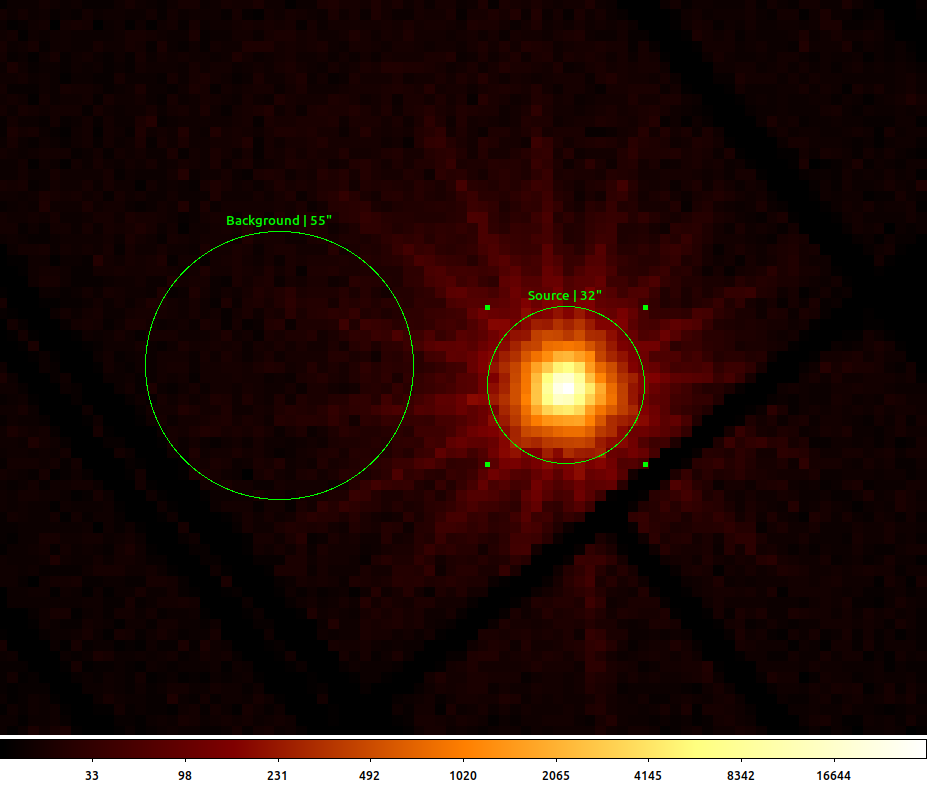
\includegraphics[width=0.8\textwidth]{images/rx-j0925-7-4758_0111150101_src-bkg.png}
		        \caption{Source and background extraction regions for the XMM-Newton observation of \source}
		        \label{fig:src-bkg:pn}
		    \end{figure}
		    
		    The source photons were idensified using DS9 and extracted from a circular region having a radius of 30" which is centred at the \source\ centroid position, encompassing about 85-90\% of XMM-Newton's telescope's on-axis PSF\footnote{\url{https://xmm-tools.cosmos.esa.int/external/xmm_user_support/documentation/uhb/onaxisxraypsf.html}}. For the background photons, first the SAS task \texttt{ebkgreg} was executed to obtain an optimum circular background extraction region of radius $\sim$55". The resulting source and background extraction regions are displayed in figure \ref{fig:src-bkg:pn}. The RMF and ARF were generated using the standard SAS tasks \texttt{rmfgen} and \texttt{arfgen}. The spectrum was finally binned to have a minimum of 10 counts/bin using the task \texttt{grphha} in order to make it ready for analysis using XSPEC.

    	
    	\subsection{ASCA SIS1 Data Reduction} \label{multi-obs:red-analysis:sis1}
    		\source\ was observed by the SIS1 instrument on-board Japan's ASCA observatory for a total duration of $\sim 21$ ks on 22 December 1994, with the purposes of characterization of its continuum spectral shape and the investigation of absorption edge features \cite{ebisawaAsca2001ApJ}. Because SIS1 has greater effective area for energies $<1.5$ keV\footnote{\url{https://heasarc.gsfc.nasa.gov/docs/asca/newsletters/sis_overview.html}}, the data analysis was restricted to an energy range of 0.2-1.0 keV. The procedures for the extraction of spectra were performed using \textit{XSELECT}\footnote{\url{https://heasarc.gsfc.nasa.gov/ftools/xselect/}} version 2.5, a multipurpose tool for filtering event files and generating images, spectra, and light curves made available as part of HEASoft.
    	
    		The event files were downloaded from HEASARC. They were loaded into XSELECT and the source and background spectra were extracted using a circular region of radius 127" and an annular region of radii 129" and 210" respectively, centred at \source\ centroid position. The RMF and ARF were generated using the FTOOL tasks \texttt{sisrmg}\footnote{\url{https://heasarc.gsfc.nasa.gov/lheasoft/ftools/fhelp/sisrmg.html}} and \texttt{ascaarf}\footnote{\url{https://heasarc.gsfc.nasa.gov/lheasoft/ftools/fhelp/ascaarf.html}} respectively. The spectrum set was grouped and binned to a minimum of 20 counts/bin using \texttt{grppha} so as to analyse using XSPEC.
    	
    	\subsection{Chandra ACIS Data Reduction} \label{multi-obs:red-analysis:acis}
    		\source\ was observed during 14 November 2000 for a duration of $\sim 57$ ks using the High-Energy Transmission Grating Spectrometer (HETGS) on-board NASA's Chandra X-ray Observatory \cite{beardaChandra2002AA}. The photons were detected with the ACIS-S CCD array at the focal plane. The data analysis was performed in the energy range 0.4--1.0 keV, with 0.4 keV being the lower limit of the HETGS+ACIS-S spectrometer combination. The extraction of the spectrum and response files was performed using \textit{CIAO} version 4.10 and the Chandra calibration database \textit{CALDB} version 4.7.7.
	    	\begin{figure}[!htb]
		        \centering
		        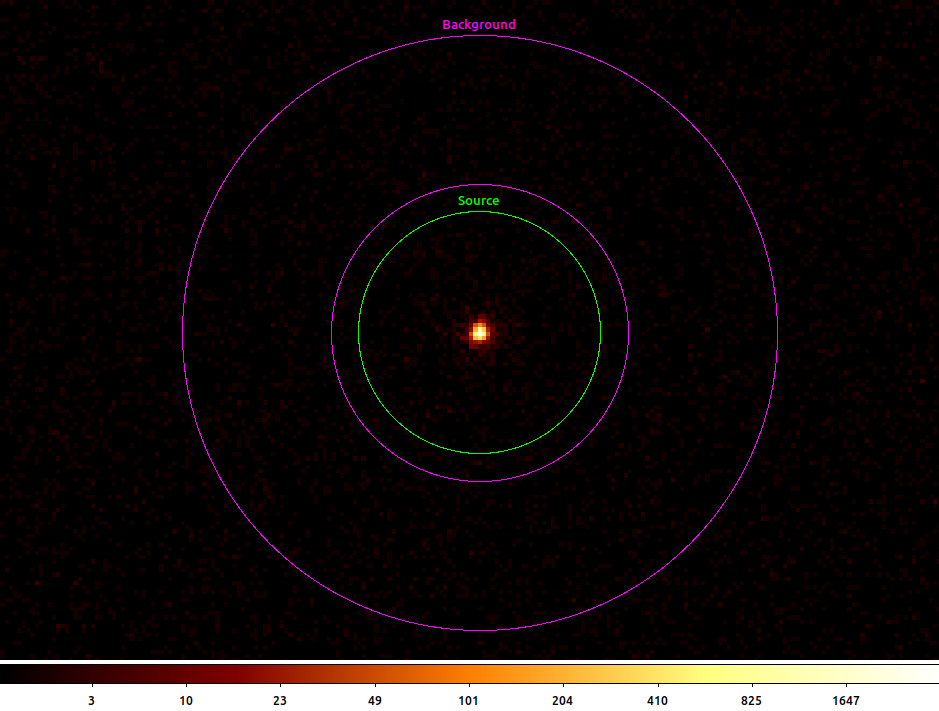
\includegraphics[width=0.45\textwidth]{images/rx-j0925-7-4758_644_src-bkg.png}
		        \caption{Source and background extraction regions for the Chandra observation of \source}
		        \label{fig:src-bkg:acis}
		    \end{figure}
	    	
	    	All the science data files were downloaded from HEASARC. DS9 was used to identify the source and background regions as being a circular region of radius 0.23' and an annular region of radii 0.28' and 0.57' respectively. The source and background spectra were extracted as FITS files using the task \texttt{specextract}\footnote{\url{https://cxc.cfa.harvard.edu/ciao/ahelp/specextract.html}} using standard parameters as per the data analysis threads for point-like sources\footnote{\url{https://cxc.cfa.harvard.edu/ciao/threads/pointlike/}}. The relevant RMF and ARF were generated using the \texttt{mkacisrmf}\footnote{\url{https://cxc.cfa.harvard.edu/ciao/ahelp/mkacisrmf.html}} and \texttt{mkarf}\footnote{\url{https://cxc.cfa.harvard.edu/ciao/ahelp/mkarf.html}} tasks respectively. The spectrum set was grouped and binned to have a minimum of 10 counts/bin using the task \texttt{grphha} for subsequent analysis using XSPEC.
    	
    	\subsection{NICER XTI Data Reduction} \label{multi-obs:red-analysis:xti}
    		\source\ was observed by the XTI instrument on-board the NICER observatory on the International Space Station (ISS) for a total duration of $\sim 21$ ks on three occasions during 18--19 May 2019. All data reduction commands for the science data were performed using NICER-specific tasks are made available with the latest versions of HEASoft\footnote{\url{https://heasarc.gsfc.nasa.gov/docs/software/heasoft/}}.
    	
	    	The XTI observation dataset and auxiliary files were downloaded from HEASARC. In order to prepare the data for processing, we set up the remote access of the HEASARC CALDB by following the recommended procedure\footnote{\url{https://heasarc.gsfc.nasa.gov/docs/heasarc/caldb/caldb_remote_access.html}}. The cleaned event files were extracted using the \texttt{nicerl2} command\footnote{\url{https://heasarc.gsfc.nasa.gov/lheasoft/ftools/headas/nicerl2.html}}. They were then loaded into XSELECT. This produces the source and background spectrum files in FITS format. The ARF and RMF were generated with the extracted source spectrum files using the \texttt{nicerarf}\footnote{\url{https://heasarc.gsfc.nasa.gov/lheasoft/ftools/headas/nicerarf.html}} and the \texttt{nicerrmf}\footnote{\url{https://heasarc.gsfc.nasa.gov/lheasoft/ftools/headas/nicerrmf.html}} commands respectively. The spectrum set was finally grouped and binned to a minimum of 10 counts/bin using \texttt{grphha} and made ready for analysis using XSPEC.
    	
    \section{Results} \label{multi-obs:results}
    
    	\subsection{Observed Count Rates} \label{multi-obs:results:count-rates}
    	
    	\subsection{NLTE Continuum Model} \label{multi-obs:results:nlte}
    	
    	\subsection{Unfolded Spectra} \label{multi-obs:results:unfolded}
    	
    	\subsection{Luminosity versus Effective Temperature} \label{multi-obs:results:L-vs-Teff}
    	
    	\subsection{Presence of Elemental Absorption Edges} \label{multi-obs:results:abs-edge}
    	
    \section{Discussion} \label{multi-obs:discussion}
    
    	\subsection{Best-fit Continuum Model} \label{multi-obs:discussion:cont-mod}
    	
    	\subsection{NLTE Pure H Model Atmosphere} \label{multi-obs:discussion:nlte-pureH}
    	
    		\subsubsection{Structural Equations}
    		
    		\subsubsection{Numerical Solution using ALI}
    	
    	\subsection{Inferences from Results} \label{multi-obs:discussion:inference}
    	
    	\subsection{Relative Strengths of Absorption Edges} \label{multi-obs:discussion:abs-edge-strength}